
\chapter{Description of data}

%%%%%%%%%%%%
%%% 2.1) %%%
%%%%%%%%%%%%
\section{Tanzania data set}

\subsection{Study site}

Data were collected as part of a program investigating the burden of the disease and its' transmission intensity, with several demographic and populational indices gathered to study and possibly predict the intensity of malaria transmission \cite{drakeley2005altitude}. The study area ranged from the highest mountain in Africa -- Mt. Kilimanjaro -- to Tanga, a coastal plain of North-East Tanzania (figure \ref{fig:2.1}). In this delimited region, six transects were defined based on the altitude -- 3 in the Kilimanjaro region, and 3 in the Tanga region -- each one containing four villages, one at high altitude ($>$1200m), two at intermediate altitude (600m$-$1200m), and one the closest to a low altitude ($<$600m), chosen to represent areas of varying transmission intensity, based on the premise that an effect of increasing altitude follows a reduction in vectors density \cite{bodker2003relationship}. For each village a selection criteria was used to minimise differences within transects in ethnicity, seasonal migration or access to health care.

% IS IT WORTH IT TO WRITE THIS PARAGRAPH?
According to the source article \cite{drakeley2005altitude}, the study area was mapped making use of differential global positioning satellite techniques (Trimble GeoExplorer III and Pro XR receivers; Trimble Navigation), and geographical data were analysed by use of Arc/Info~7.1 and ArcView~3.2 (ESRI). The long-term average daily mean temperature was derived from meteorological stations across both regions and rainfall estimates were derived by Meteosat infrared data collected by the Climate Prediction Center at the US National Oceanographic and Atmospheric Administration.

\begin{figure}[ht!]
\center
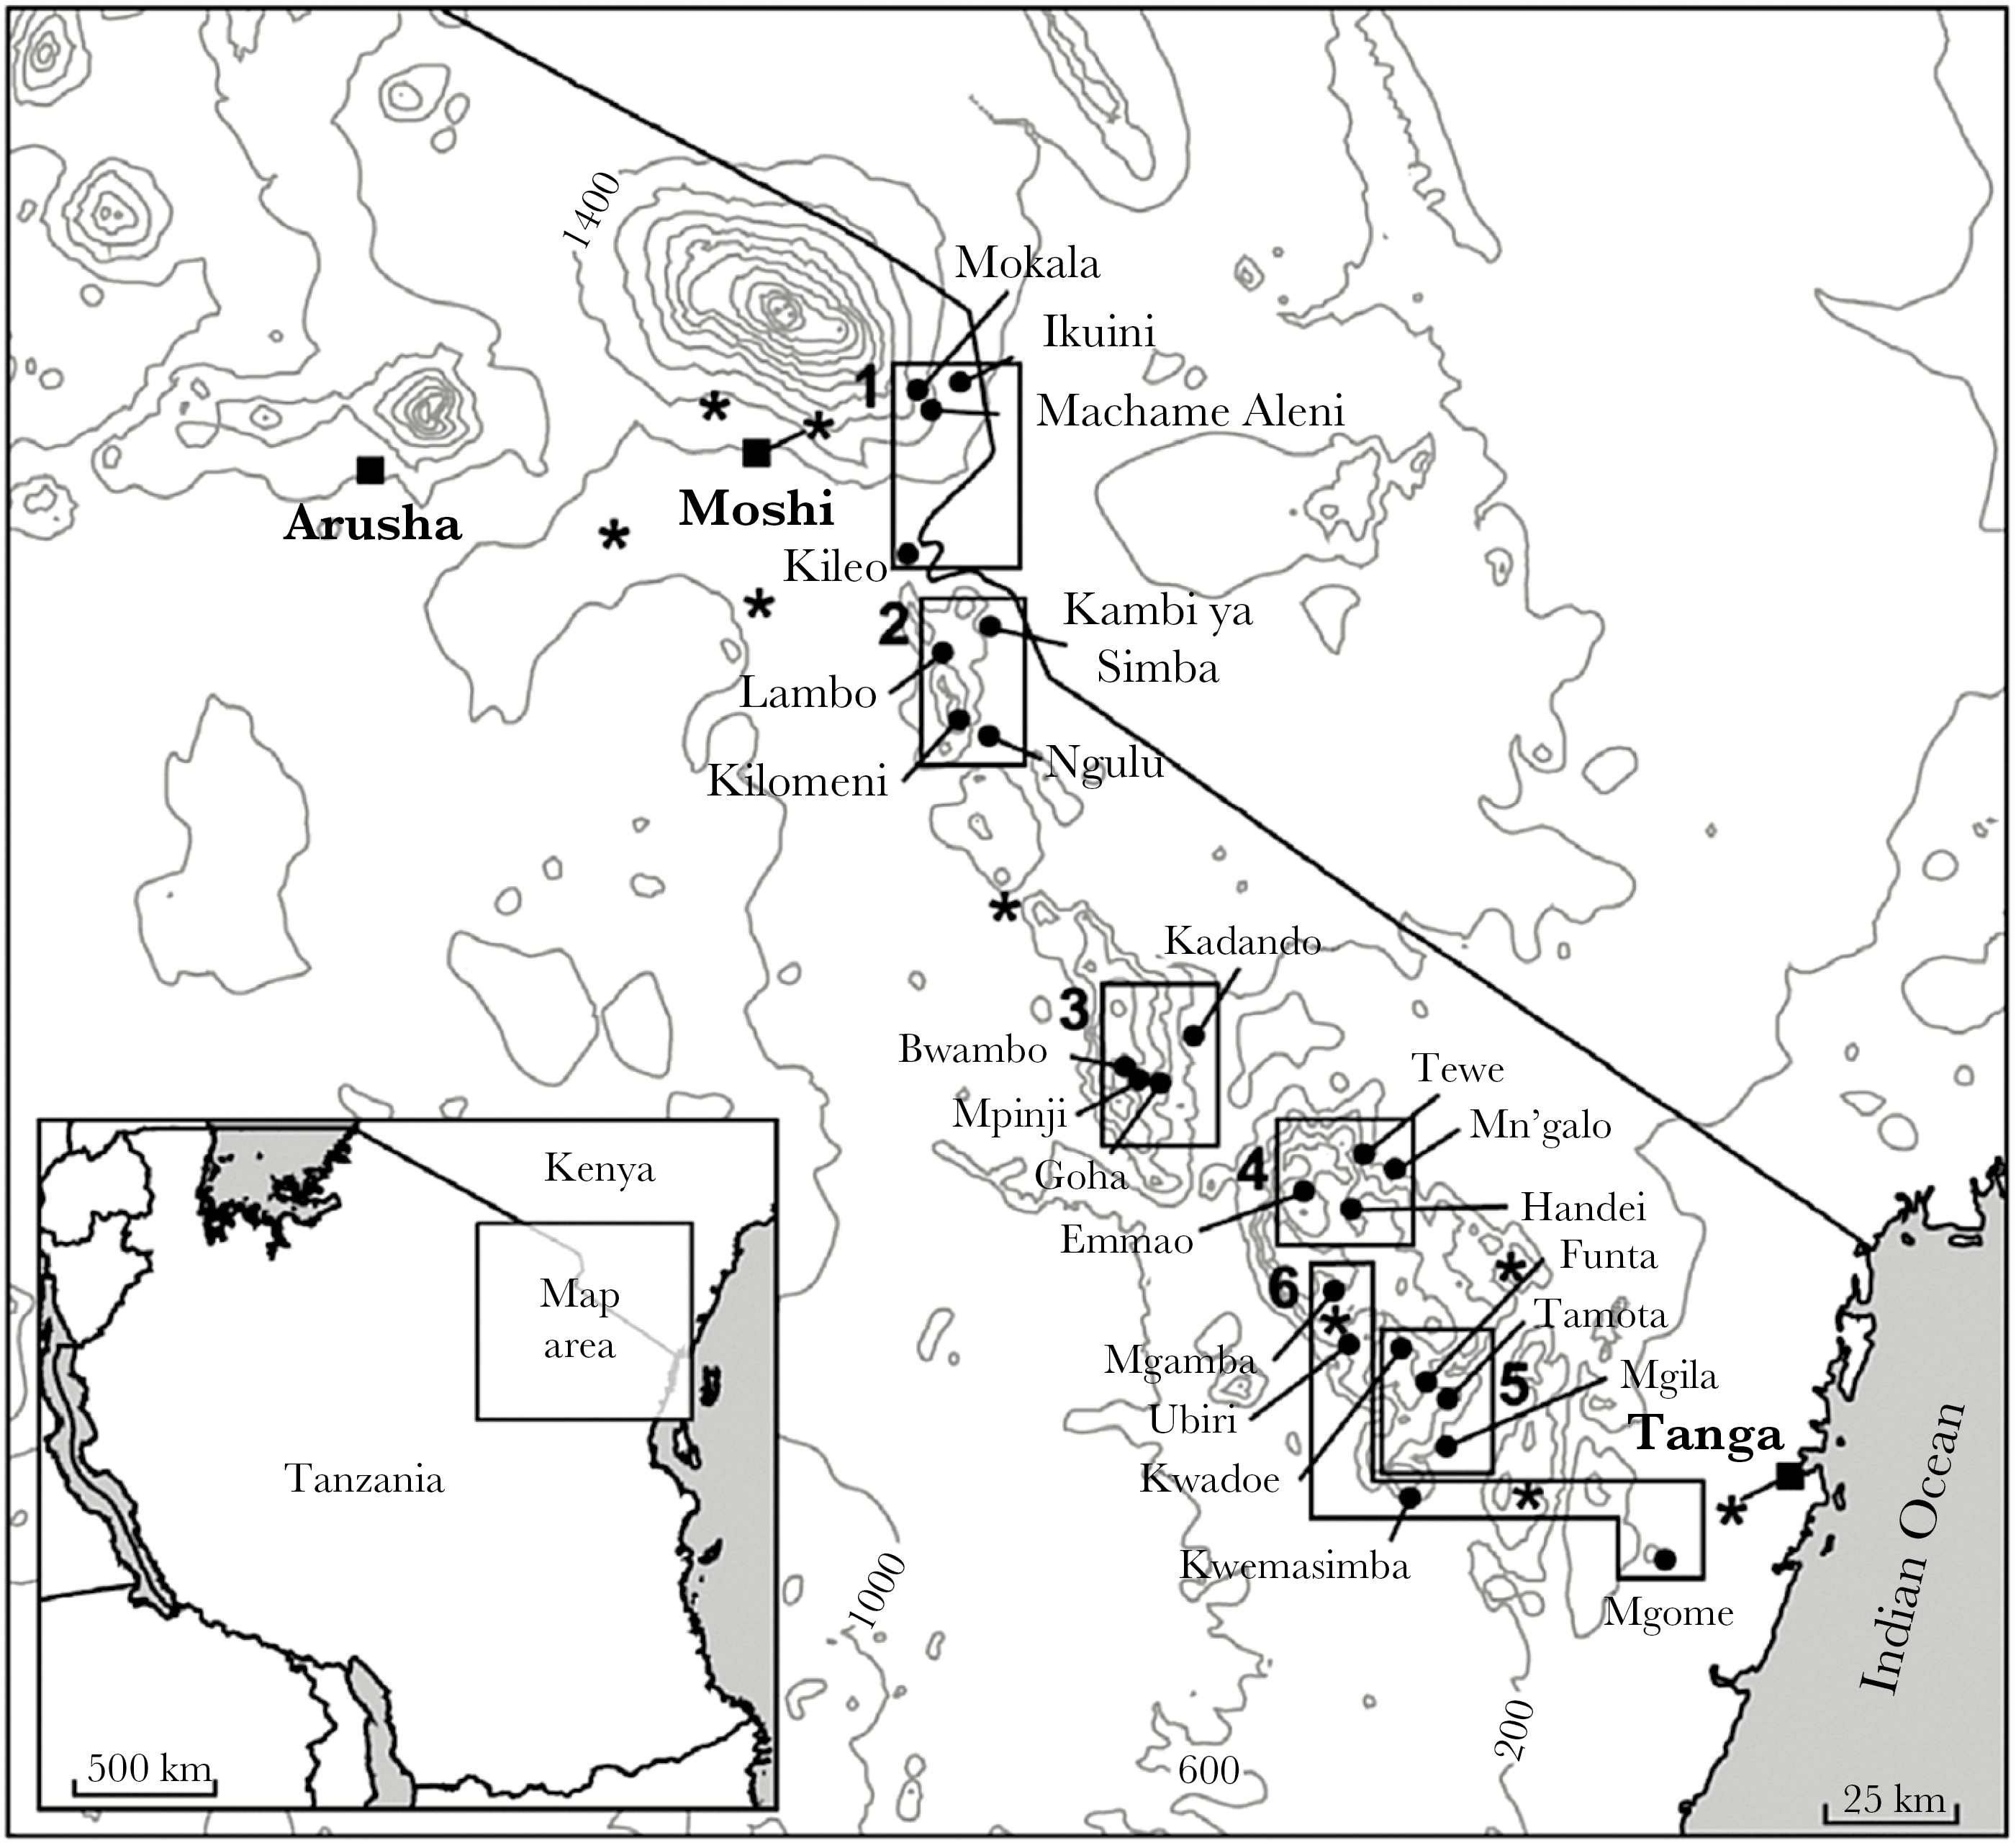
\includegraphics[width=13cm]{images/site_map.jpeg}
\caption[Map of study sites]{Map of study sites (black circles) grouped by respective numbered region transects: Rombo (transect 1), North Pale (transect 2), South Pale (transect 3), West Usambara 1 (transect 4), West Usambara 2 (transect 5) and West Usambara 3 (transect 6). Locations of the 8 meteorological stations are also shown (asterisks).}
\label{fig:2.1}
\end{figure}

\subsection{Cross-sectional surveys}

Two cross-sectional age-stratified malariometric surveys were conducted in each village after the short rainy season in November 2001 and again the following year in June, after the long rains. The study collected blood samples, as well as anthropometric and clinical data from a total of 250 villagers, with the number of individuals structured by age, 80 who were 0$-$4 years old, 80 who were 5$-$14 years old and 90 who were 15$-$45 years old. For the survey, attention so that the sexes were equally represented was taken, being achieved in the younger age groups, although 70\% of the 15$-$45 years old surveyed were woman.

The study was able to collect several demographical values (altitude levels, estimated daily temperatures, estimated annual rainfall) for each one of the 24 villages), as well as specific and proportioned age-stratified information for the different populations, including individual values such as age, gender, marital status, height, weight, body temperature, haemoglobin levels, presence/absence of malaria infection and specific antibodies to the malaria antigens.\\
Due to the variety and quality of such information, this data set has been used on multiple different studies with the focus being serological analysis, inquiring about the trends in malaria endimicity \cite{drakeley2005estimating}; genetic studies on populations exposed to \textit{P. falciparum} parasite \cite{enevold2007associations,sepulveda2017malaria}; and development of specific mathematical model, used for serological analysis \cite{bosomprah2014mathematical}.

%%%%%%%%%%%%
%%% 2.2) %%%
%%%%%%%%%%%%
\section{Data processing}

%All statistical analysis were performed in the software R version 3.4.1.\\
Having such large collection of variables, it's necessary to perform some filtering (the ugliest sentence ever written \dots). For the purposes of this analysis, specific variables were selected, and the two different times registered were unconsidered.\\
Demographic and epidemiological variables for this analysis were: transect, village and its' ID, village mean altitude, ethnic groups, gender, age in years and the respective age group, presence of \textit{P. falciparum} malaria infection and results from three specific antigens for the disease. The decision to perform the analysis using only the complete cases for the described variables let to the removal of three villages from the transect West Usambara 3 due to the lack of values for the antibodies. This last transect was reduces to the Mgome, the village with lowest altitude where such values happened to be collected.
 
\subsection{Variables description}

\subsubsection{Dependent variable}

To study the levels of infection among Tanzania's population, the presence/absence of \textit{P.falciparum} malaria was considered as the response variable. Having a Bernoulli distribution, this variable takes the value $0$ whenever there's no detection on malaria infection in a screened individual, and $1$ if the individual is reported as infected with the malaria parasite. This response variable has a direct use to estimate the proportion of disease as well as prevalence rate of the population.

\subsubsection{Covariates}

Having been collected with different methodological objectives (is this true? can I admit this?), the selected covariates were grouped in two distinct groups: demographical and epidemiological.

\begin{enumerate}
\item Demographical variables 
\item Epidemiological variables -- Antibodies and antigens. Exposition markers \textit{vs.} protection markers. Antibody relation to the prevalence.
\end{enumerate}

\textbf{Aqui inserir tablelas e tudo o resto para a análise descritiva!}

\subsection{Antibodies possible cross-reaction}

Existence of correlation between antibodies. First important conclusion: existence of cross-reaction! Correlation map!
